\documentclass[UTF8]{ctexart}
\usepackage{../Zhihu}
\usepackage{mhchem}
\title{数字电路学习笔记(十二):时序逻辑设计}
\begin{document}
\maketitle
\begin{figure}
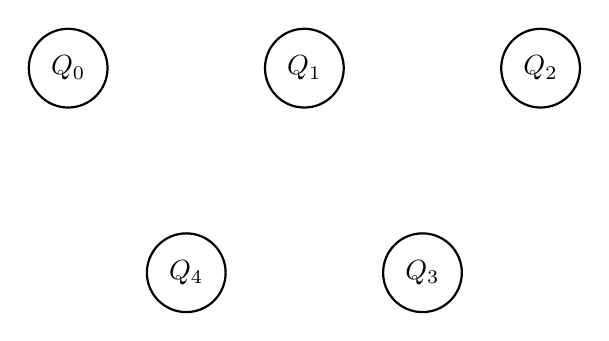
\begin{tikzpicture}[scale=1]
    \draw[thick] (0,0) node {$Q_0$} circle[radius=0.5];
    \draw[thick] (3,0) node {$Q_1$} circle[radius=0.5];
    \draw[thick] (6,0) node {$Q_2$} circle[radius=0.5];
    \draw[thick] (1.5,{-sqrt(27)/2}) node {$Q_4$} circle[radius=0.5];
    \draw[thick] (4.5,{-sqrt(27)/2}) node {$Q_3$} circle[radius=0.5];
\end{tikzpicture}
\end{figure}
\end{document}
